\chapter{CEMicro Architecture and Technology Stack}
\label{sec:arch}

How was the "is" sutation when starting?

How should it look like?

How do I get there?


\section{The existing appliction}

The existing application which this department of Capgemini is working on in a point of sales (POS) software. It is essentially the toolkit a salesman uses to create an offer for a potential customer. Since cars are a highly configurable product the POS software has to support a huge variety of options, made even more complex by the different types of cars, different types of brands, or sub-brands, and the fact that it is used across several markets and languages. Each market has its very own requirements and also their levels of hierarchy which have to be reflected within the application in terms of user management and access levels.

The part of the application which involved my task is the creation of the final offer as a printable PDF document. Depending on the object of the sale, the type of car, the current market and a host of other factors the application will decide which document template to use and will collect the appropriate lines of text and values from the database to assemble into a finished document which is then generated in the PDF format. Additionally, there are several configuration pages in the admin area of the application where these templates can be managed and the contents defined. Figure \ref{fig:pos} shows a glimpse of the rather unwieldy admin interface for the part of the document creation.

There are currently six teams of about eight developers each working on the POS application.

\begin{figure}
  \centering
  \begin{subfigure}[b]{0.5\linewidth}
    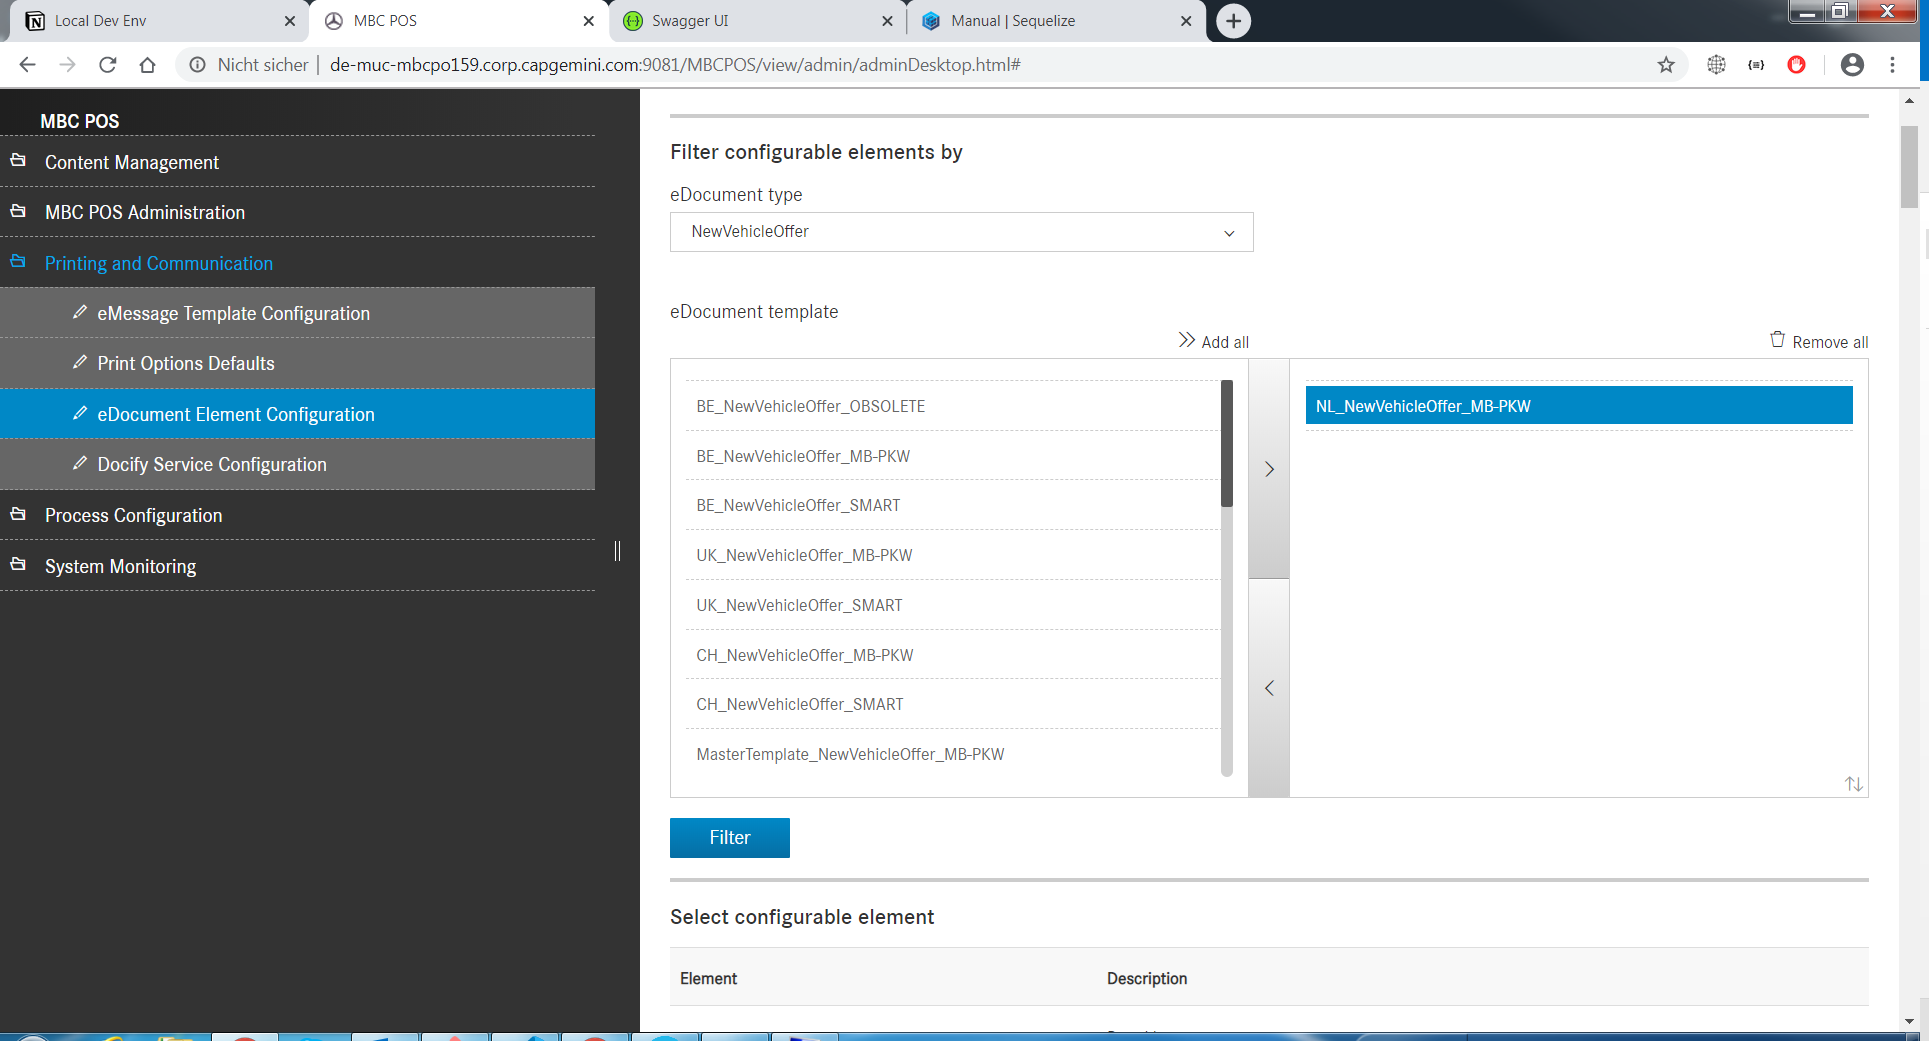
\includegraphics[width=\linewidth]{assets/pos-ce-config-1.png}
    \caption{Template selection}
  \end{subfigure}
  \begin{subfigure}[b]{0.5\linewidth}
    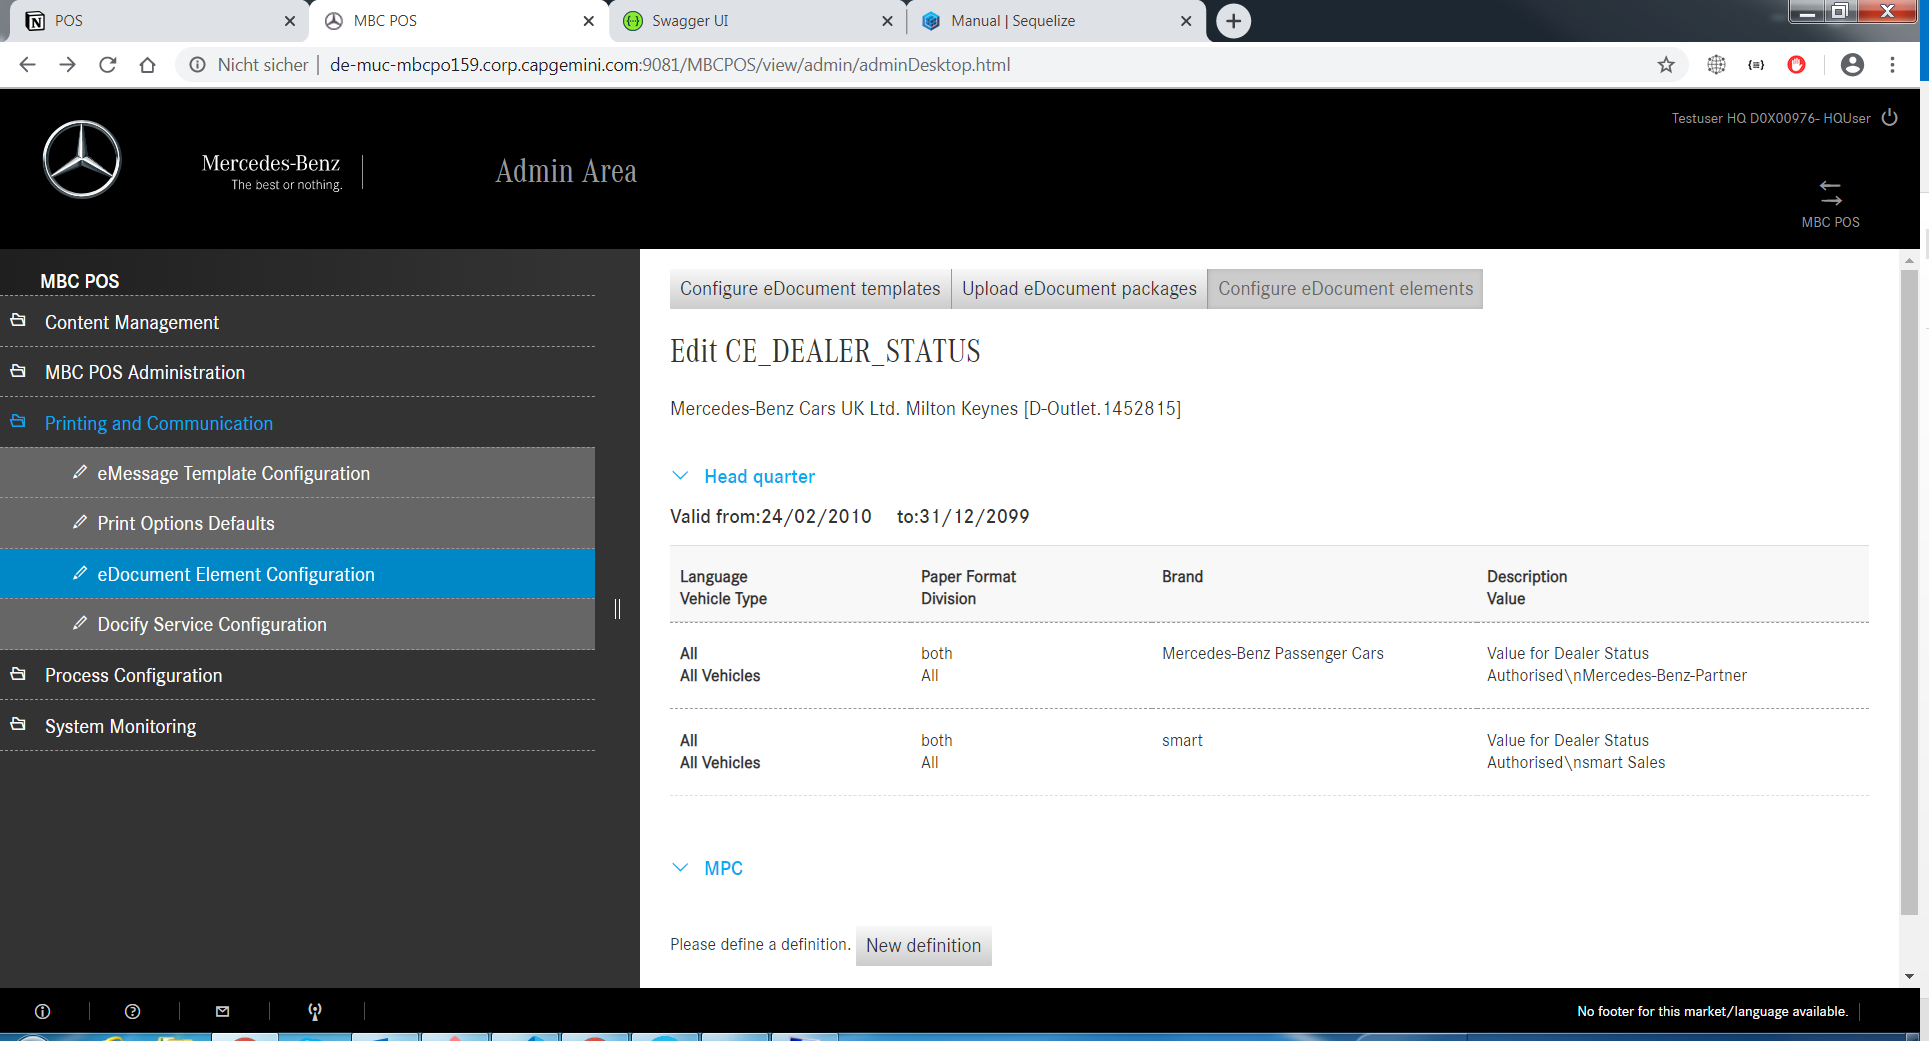
\includegraphics[width=\linewidth]{assets/pos-ce-config-3.png}
    \caption{One CE contains several children}
  \end{subfigure}
  \caption{POS configurable element admin page}
  \label{fig:pos}
\end{figure}

The part of the application responsible for generating a printable document has been part of a past student project very similar to my task. The team of students built essentially a microservice that is responsible for managing the templates and which can be called through an application programming interface (API) which returns the finished PDF. This service was named Docify.

Docify is a kind of textbook example for a microservice. A document printing service lends itself very nicely to be extracted into its separate application because its interface is so clearly defined. The interface for a printing service requires two properties, first, the name or identifier of the predefined template and second, the dataset which is needed to fill the gaps of the template. That means often the biggest challenge for distributed services, defining the boundaries and thus their interfaces are no-brainers for this use-case.

Figure \ref{fig:docify} shows the administration interface for Docify and it is easy to see how each of the two previously mentioned API criteria has their page. On the left (a) is the list of template identifiers, each template is identified by a client-market-name tuple, and on the right (b) is the editor for template specific templates with the HTML representation on the left and the rendered preview. The HTML code contains several placeholders which will be replaced by their respective value when the document is printed out.

\begin{figure}
  \centering
  \begin{subfigure}[b]{0.5\linewidth}
    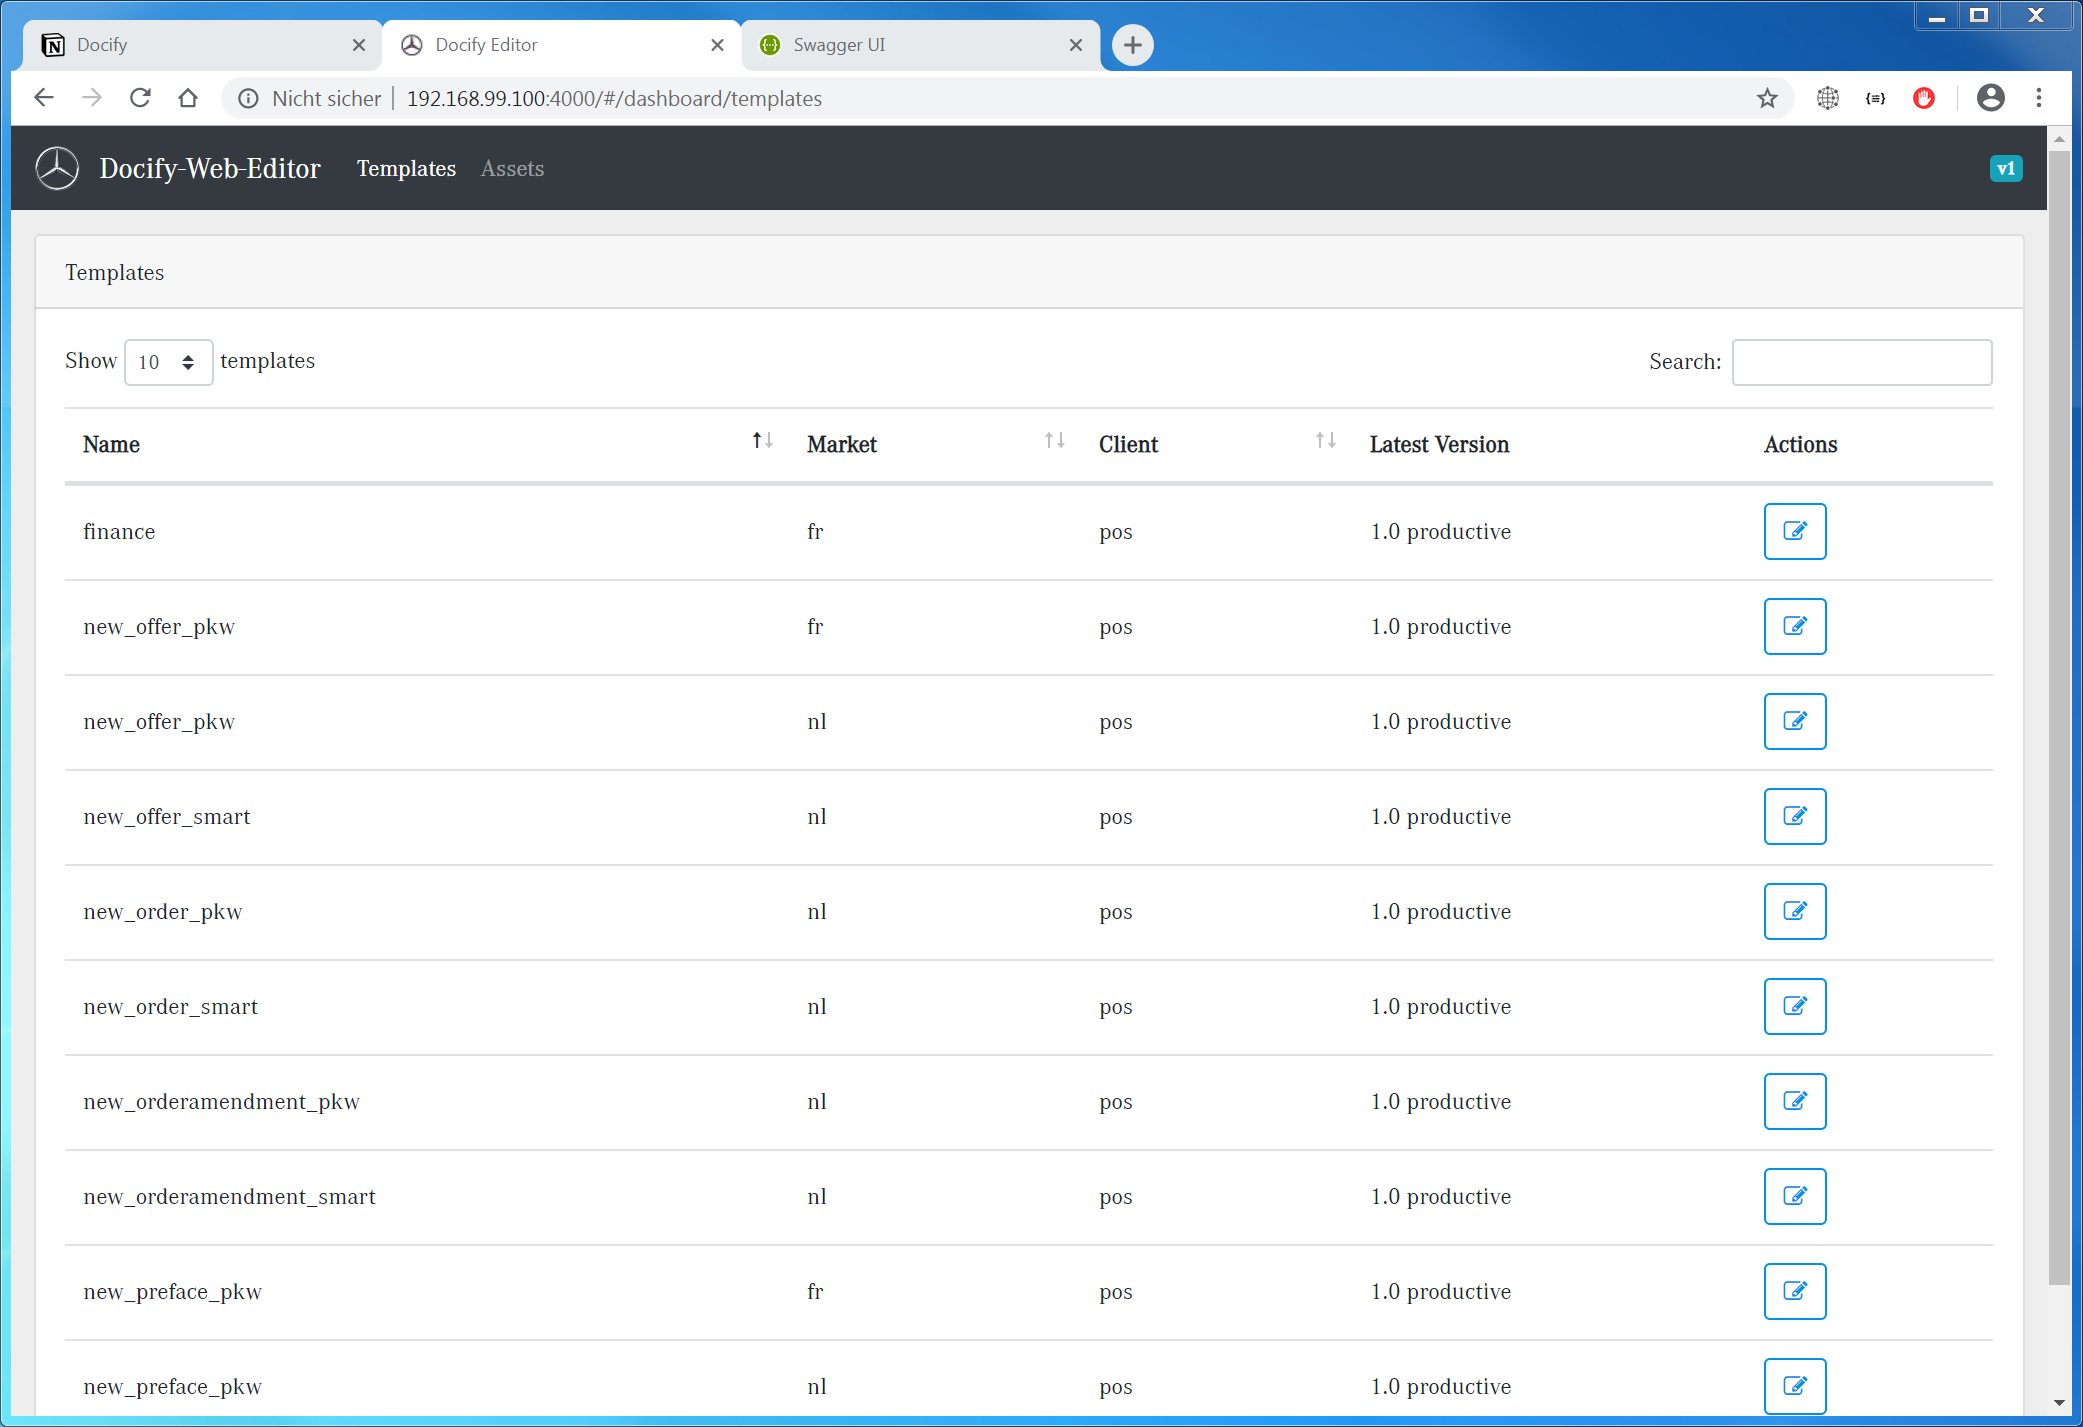
\includegraphics[width=\linewidth]{assets/docify-template-list.png}
    \caption{Template list}
  \end{subfigure}
  \begin{subfigure}[b]{0.5\linewidth}
    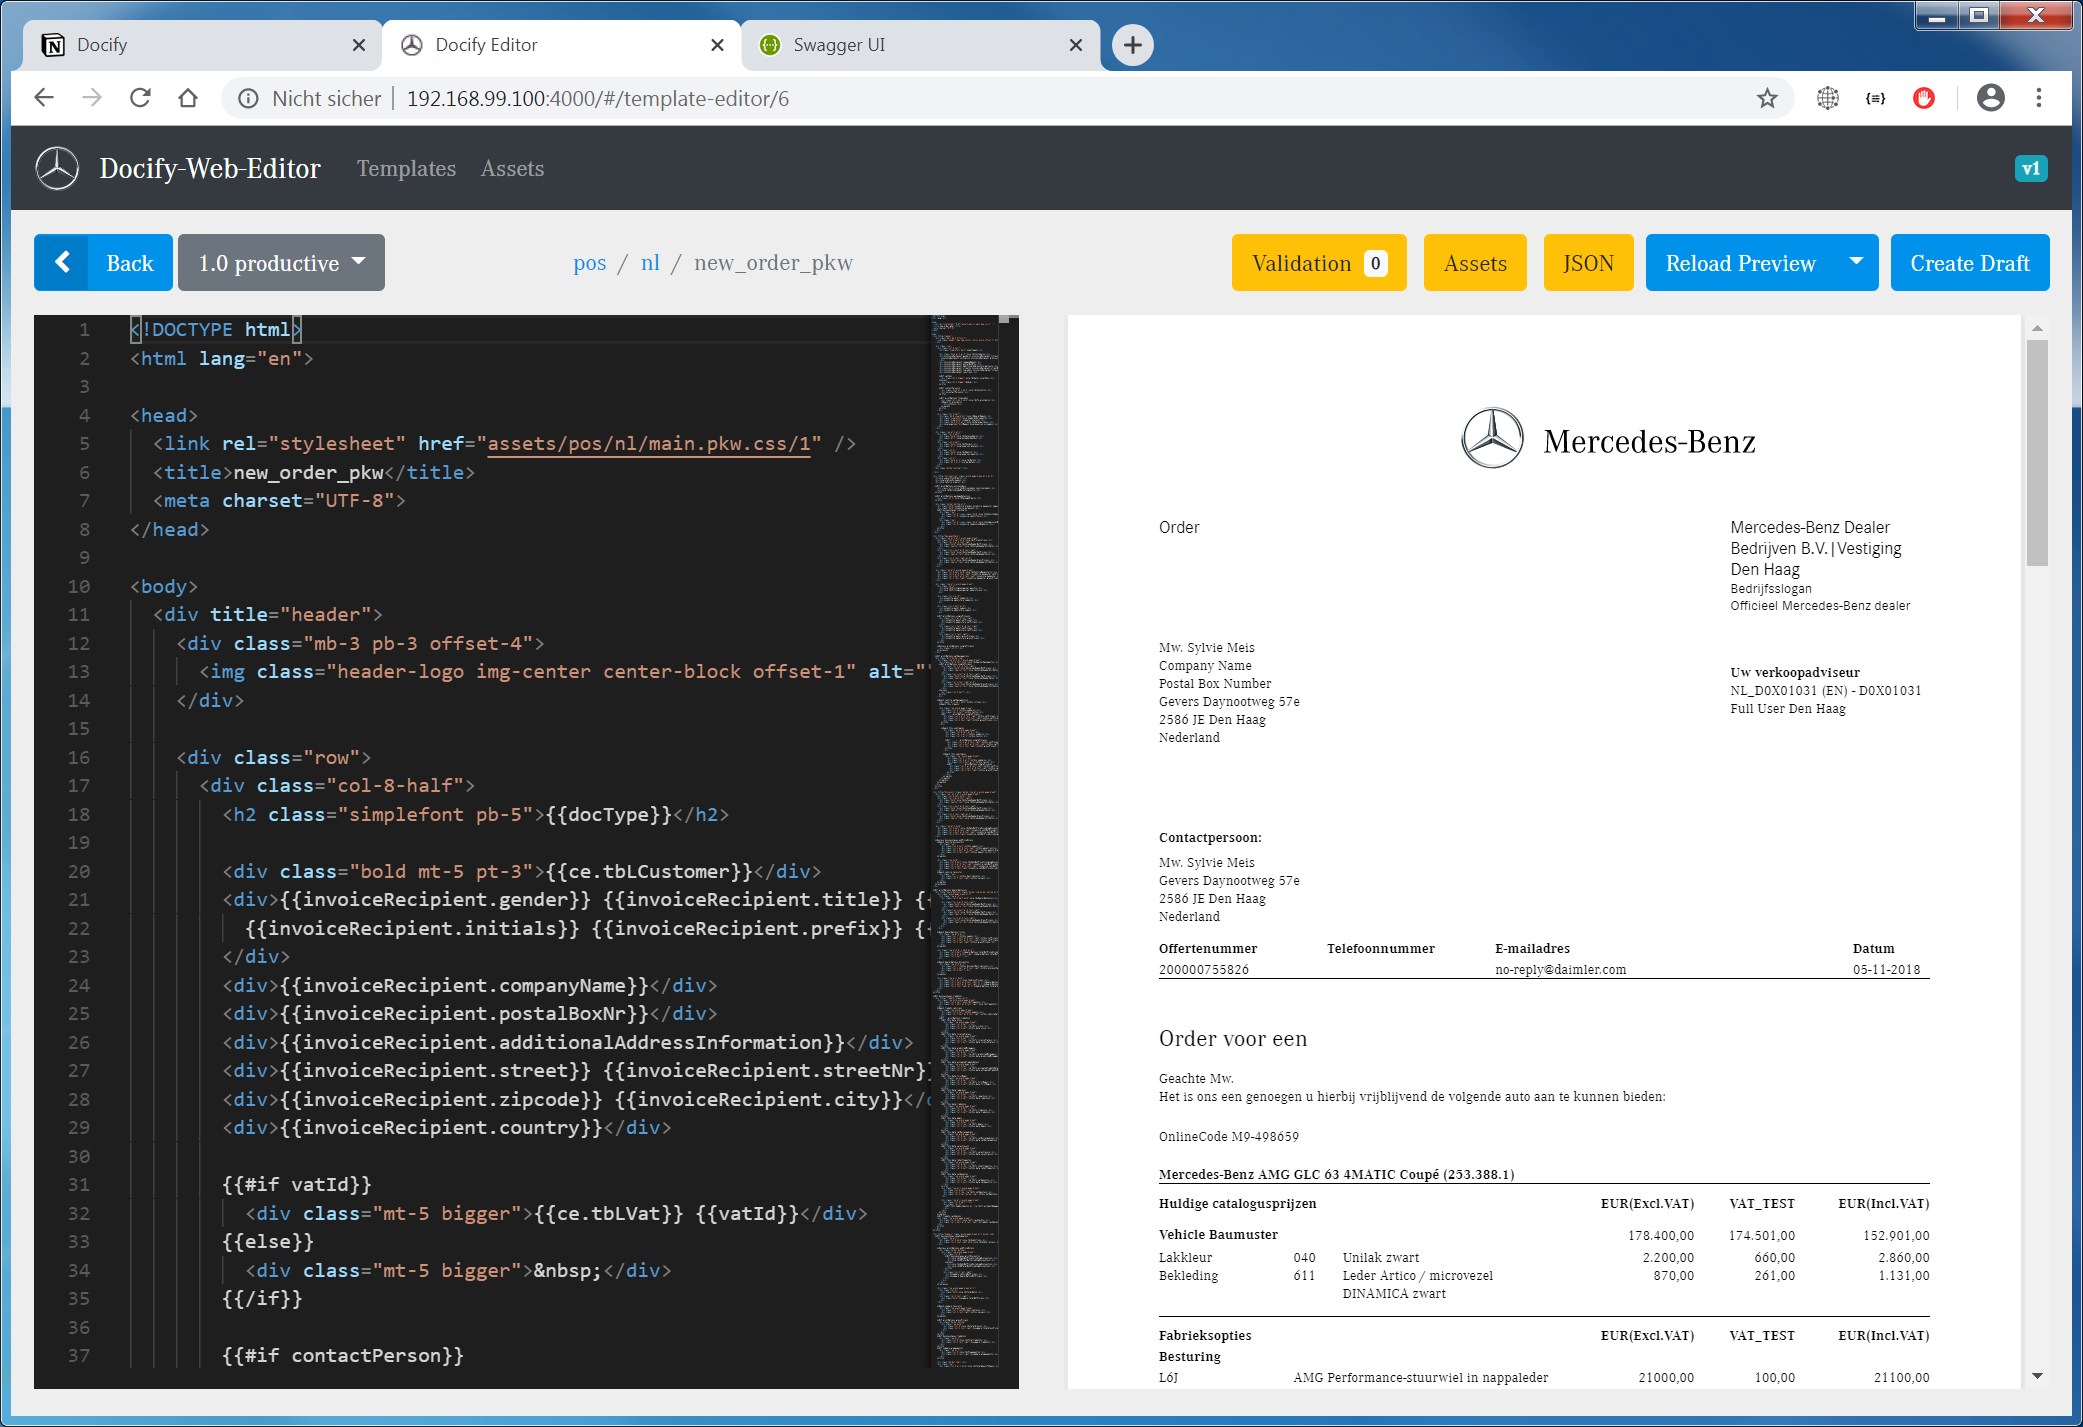
\includegraphics[width=\linewidth]{assets/docify-editor.png}
    \caption{Template editor}
  \end{subfigure}
  \caption{Docify template editor app}
  \label{fig:docify}
\end{figure}

While the technical aspect of Docify might be simple it is interesting to observe the non-technical challenges that a microservice is facing. Besides the question of how a microservice should be extracted and build there is the economic question of why it is necessary to invest the time into building such a service when it seems to be working just fine as it is. The question every project has to face is "Does it add business value?", and if it doesn't, why should the business spend money on the project? This is an interesting question especially for engineers who often try to build the ideal solution for a problem, after all, that's why we became engineers in the first place, but forget that our time is valuable and to build the ideal solution, in this case, a microservice, for an already working feature may not make much sense to the business as a whole.

So why was Docify build in the first place? I haven't been involved myself but from the proceedings with my project, I can surmise some good indicators. On the one hand, the POS application is over five years old, which in the world of software is a man with a cane and a white beard. Over the lifetime of an application, it tends to become ever more complex and both in its technical scope but also in terms of management. Thus even small changes to the codebase can take several days or even weeks until the task gets prioritized, implemented and deployed. In the ideal situation, the database contains all the parts which users are supposed to be able to edit so that changes don't have to be handed to developers, but in the case of POS, many adjustments to the document creation could only be done by direct manipulation of the codebase which meant that a task hat to be created for developers.

One example of this directly involves my task, the so-called "Configurable Elements" which I will describe in more detail in the next section are essentially texts that can be edited by users. But the definition for these elements is hardcoded in the application, meaning if users want to add a new such element they have to create a task for devs to do so, which adds considerable friction to a task which should be just one click. Essentially, Docify enables users to do administrative tasks directly while saving all the development time of adding these admin interface features to the existing monolith codebase.

The other business value has to do with the fact that there is currently a certain hype around microservice architectures. The project of Docify enabled Capgemini to showcase this architectural model on a fairly simple use-case to its client while not losing much in terms of wasted development time if the client declines its further development. And since a microservice can be built in a completely separate tech stack is was essentially a proof of concept/demo of a flashy new architecture and some flashy new technology.

In the end, the client liked what business value Docify had to offer and was willing to invest in its development. At the time of this writing, Docify is two years old and was rolled out to two of the several markets POS is operating in. Meaning even after two years of development the POS team is still maintaining the old implementation in spite of the new and shiny microservice which is probably a good image of how large companies tend to operate if their internal structures became sufficiently complex.

\section{Goals of the CEMicro Service}

- What is the microservice supposed to do

- High Level Overview Illustration

- Complexity of POS / CE Properties

- Out of scope: Access control


As already noted in the previous segment the idea of a microservice for document creation is pretty straigtforward since the API is well defined from the get go. The printable document handling in POS however has three parts, besides template and dynamic values which are different on a per offer basis it defines a number of staic values inside the templates which are calles "configurable elements". The idea behind configurable values, or CEs in short, is, that they are the same on every printout, but can be defined according to a number of factors like the current language, if branded or blank paper is used, if a new or used car is sold and so on.

The next segment will go into more detail what complexity was actually hidden behind the rather simple looking CEs but suffice to say at this point, the setting of these static values for printable template is cumbersome and complicated by nature of its configurability requirements.

My task therefore was to extract the confirguration of these CE values into a seperate service which can be queried by the POS system to retreive the correct set of CE values for any given document template under a given set of conditions. Fo example, if the salseman using POS wants to print a offer for a new car in the Netherlands on blank paper the POS application would then send a request to this new service saying: "please give me all the configurable elements I need to print a new offer for this and that car in the Netherlands marked on blank paper". The responsibility of the service would then be to produce a list of key kay-value pairs that the POS application can then hand to the Docify serive, or its internal printing function for that matter, to be inserted into the configurable element placeholders in the document template.

No much guidance was given to me beyond this point from Capgemini. I was given access to the source code of both the POS application and the Docify service and could start them on personal virtual machines to understand their working. Because several teams of developers were working on POS and after seeing the size of the codebase I quickly concluded that it would not make much sense for me to try to understand the inner workings of the existing Java code. Rather I decided to investigate the user interface of both services, and in the case of Docify, the API to understand what features the my service needs to offer and what interfaces it should expose.

I decided to call the service CEMicro, short for Configurable Element Microservice. The name is rather boring and not in the vain of more modern hipster names like Spotify or Instagram, but it serves a very functional purpose in communicating quickly what it is supposed to do to an audience that is familiar with the existing cumbersome feature of configurable elements. I felt a functiona name that eases the adoption of a new service was more expedient than a nice and fancy name.

Early in the planing of the application context, that is, whith whom the new application needs to communicate about what, I assumed that CEMicro only needs to talk to the POS system since in the end only the POS system will request a dataset from CEMicro. But after understanding that the templates are actually not available to POS bur rather maintained by Docify it became clear to me that either CEMicro has to have it's own copy of each template or it needs to request the template from Docify in order to know which configurable elements the template needs. Another option would have been for users to tell CEMicro which configurable elements exist and are part of which template, but this would have ment a double effort for users since each new CE that was defined inside a template in Docify needs to be additionally added to CEMicro, which brings us to the concept of the single source of truth.

The single source of truth [ref] is a fundamental concept in programing that a value or variable should only be defined and maintained in one place, the source of truth. As soon as it is defined in multiple places, they have to have a system to keep each other synchronised otherwise the application state will be inconsistent. The single source of truth principle thus becomes even more important for a distributed service architecture. In a monolith application, and this is really the reason why monoliths are easier to develop and more widely used, there is usually only one database and the whole application has access to all the data. But in a distributed service architecture every individual service only has their individual database. In order to make this work each service can only handle the data of its particular domain and has to request the data of other services through their public interfaces. In the case of CEMicro the database can only contain the data of the actual configurable elements and not the data of the templates, or the user table for that matter. If copies of a dataset would exist in the databases of multiple services there would need to be a mechanism to keep all these copies in sync. This can be done through a publish-subscriber pattern [ref] but if the availability of the network can not be guaranteed, and the first rule of a networ is that its availability can not be guaranteed, then the data can become inconsistend between copies. And with computer systems where millions of daily requests is no rarity the rule that what can happen will happen is pretty much a given.

It was therefore decided to include both POS and Docify in the new services context. If a user wants to manage the configurable elements of a template CEMicro will request the list of available template and then the individual template from Docify, scan it for all the placeholders which will be replaced with CE values, and add a database entry for each value with an unique composite index that is comprised of the template name and the market. The user can then edit each individual configurable element which is directly persited to CEMicro's own database. POS can then request the list of configurable element values by the unique template name and market pair. Figure \ref{fig:context} shows the public interfaces of the CEMicro service, its related third party applications and its own three layer structure of database, server and client.

\begin{figure}
  \centering
  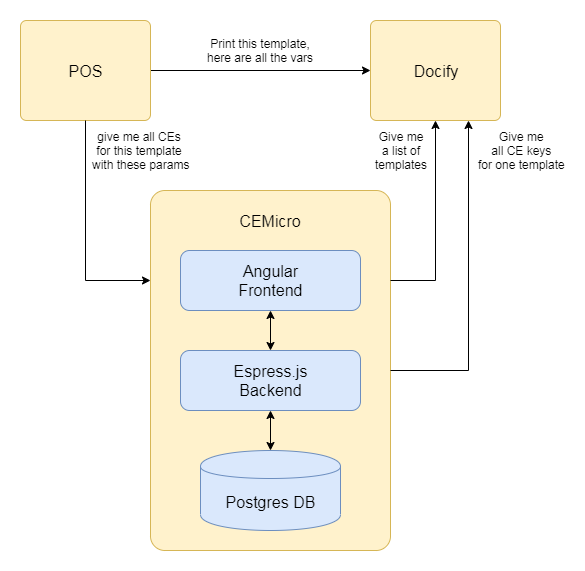
\includegraphics[width=0.6\linewidth]{assets/high-level-overview.png}
  \caption{High level context overview for the microservice}
  \label{fig:context}
\end{figure}

While the CEMicro service would become more complex than at first anticipated it was also decided to exclude some functionality from it. The reason is simply the limited time of the project, four months, and the nature of it being a proof of concept rather than a production ready application.

One feature that was decided as out of scope for this project is user management, or access control. The POS application has a fairly complex structure of access controll with its various layers of authority, starting from the so called HQ, the highest entity per market, through various levels of smaller and smaller organisational structures down to the local reseller. Each of these levels can define their own set of configuration options which may or may not be overwritten by the next lower level of management. Because access control, especially such a elaborate one, adds a nother dimension of complexity to every project, it was decided to create this proof of concept whithout any, meaning there will only be one user who has can do everything.

Another vital part of an application which was neglected is testing, both unit and integration testing. Testing is more if an implementation detail and will therefore be further discussed in chapter \ref{sec:impl}.

\section{Understanding the task}

Challenge: Understanding the task

What is a configurable element?

What properties does a CE have?

Challange/Example: Devs didn't know that CEs are not uniqe per template

\begin{figure}
  \centering
  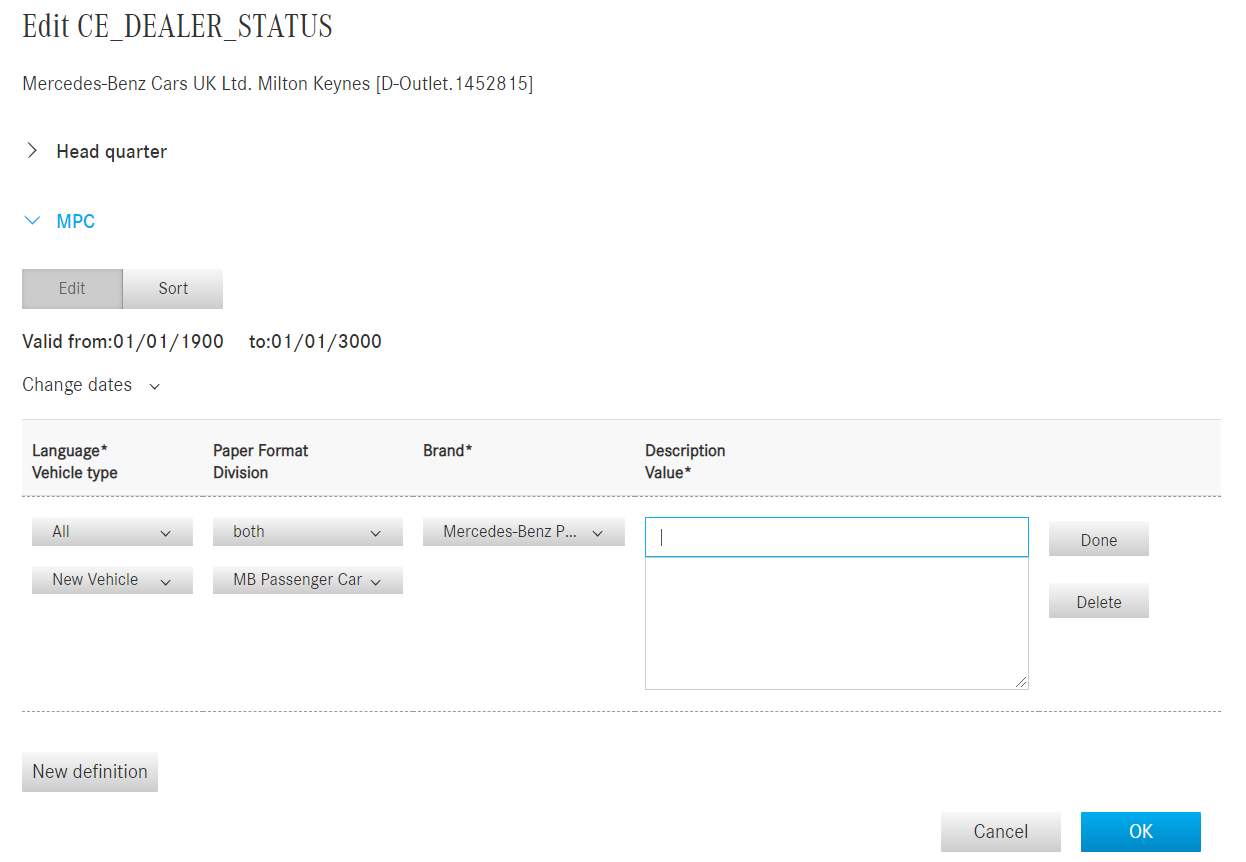
\includegraphics[width=0.8\linewidth]{assets/pos-ce-config-4.png}
  \caption{Configurable Element configuration properties}
  \label{fig:ce-properties}
\end{figure}


\section{Making optimisations}

How can the complexity of CEs be exposed in a simpler way?

\begin{figure}
  \centering
  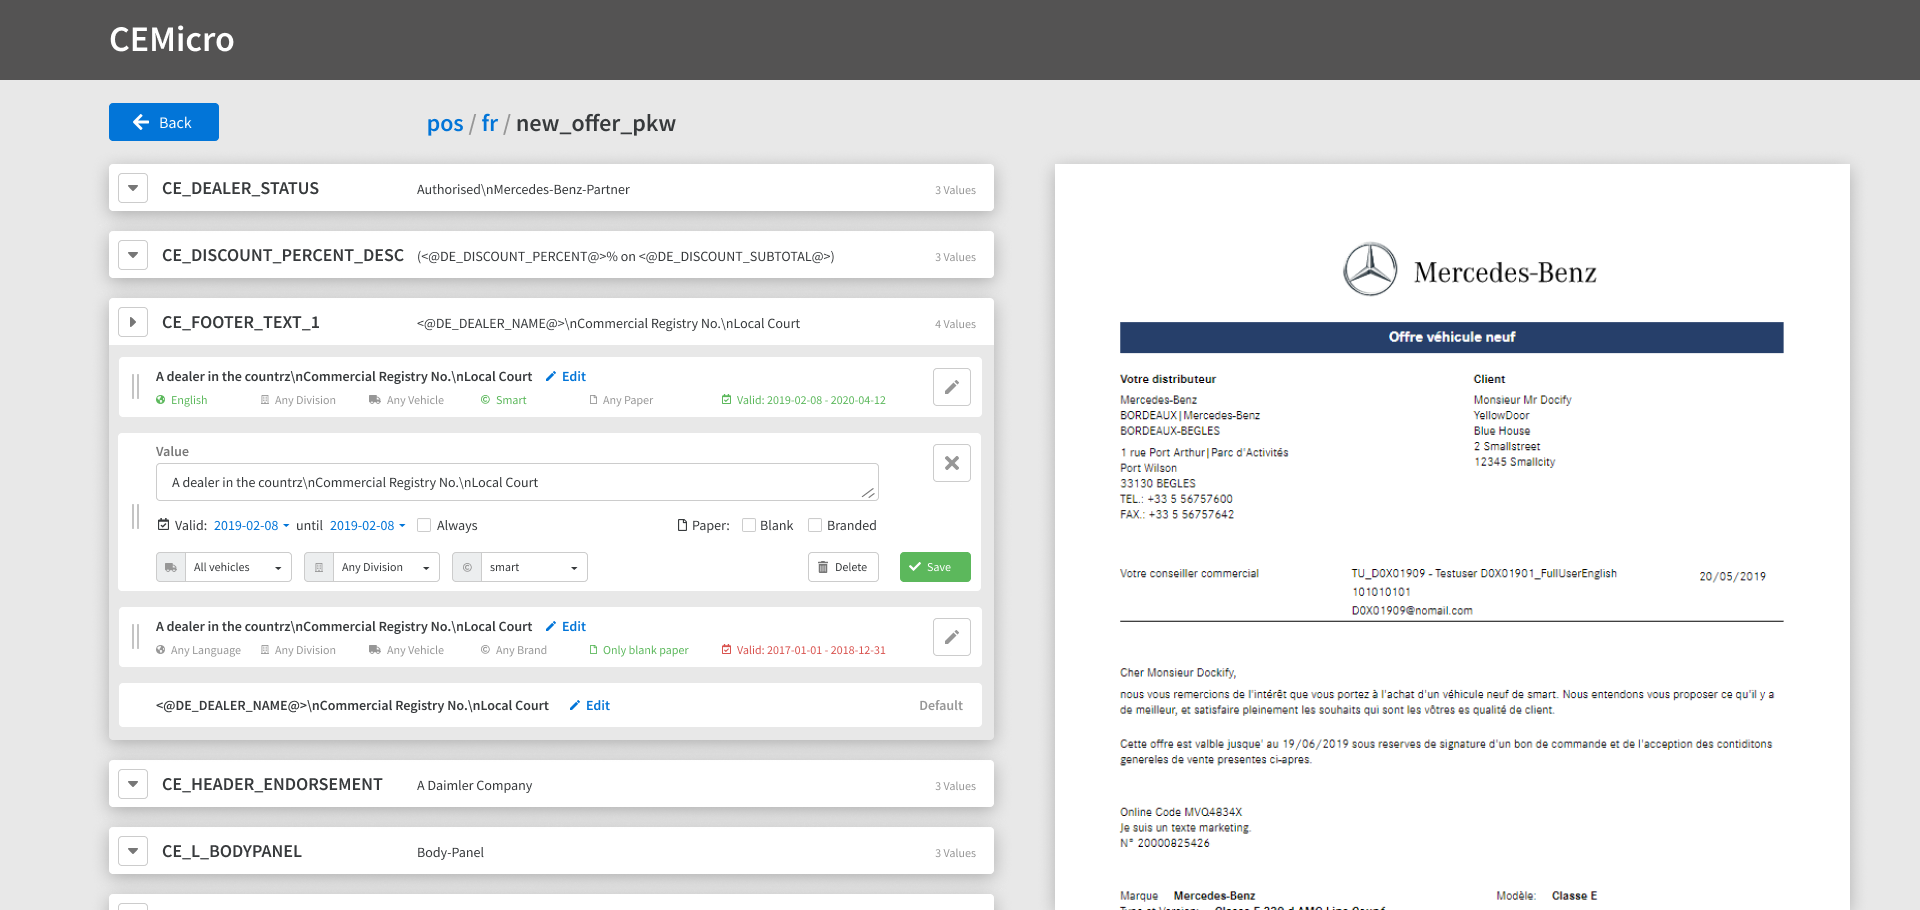
\includegraphics[width=\linewidth]{assets/cemicro-ui-mockup.png}
  \caption{User Interface mockup for CEMicro}
  \label{fig:mockup}
\end{figure}


